\section{Results}
\subsection{Tracking performance}
|Motivation why we build it|

The presented model splits the tracking problem into growth cone detection and
identity association. A representative example of detections is shown in Figure
\ref{R_modelresults} B. Given the temporal stack of five image tiles, the
detection model accurately identifies growth cones in PDMS micro structure
timelapse frames. False positive detections made by the model are often
ambiguous image regions that may be interpreted as positives under less
conservative ground truth labelling. On the test set, the detecter reaches a
precision of 0.73, and recall of 0.79. F1 score at a confidence threshold of
0.79 is 0.76 (Figure \ref{R_modelresults} C). A both deeper and wider CNN
architecture did show decreased performance. The ensuing step of identity
association was performed in a graph framework optimizing for minimum cost flow
solutions. Matching detection performance in tracking is challenging as in
addition to detection, identity switches, object occlusions, and suitable
identity creation-, and termination need to be considered. Using the multiple
object tracking benchmarks proposed in \ref{mot_benchmark}, our tracker achieves
identity precision, recall and F1 score of 0.73, 0.68, 0.71, respectively, which
is a reasonably small drop from detection performance (Figure
\ref{R_modelresults} D). The commonly used MOTA (multiple object tracking
accuracy) metric which considers the number of false positives, false negatives
(including identity), and identity switches normalized to the number of ground
truth labels was 0.61. A more intuitive measure of tracking performance is
visualized by the top bar in Figure \ref{R_modelresults} D, indicating the
proportion of growth cones mostly tracked (0.57), partially tracked (0.23), and
mostly lost (0.2). 

Although not utilized for our application of the tracking model, axons can be
reconstructed from the growth cone track, assuming that outgrowth followed the
shortest path between detections. 
% ==============================  TO-DO  =======================================
% ref suppl figure 
% ==============================  TO-DO  =======================================



\begin{figure}
    \includegraphics{R_modelresults.pdf}
    \caption[Growth cone tracking model performance]
        {Growth cone tracking model performance. \textbf{A} Loss and performance
        over 1500 training epochs. Dotted line refers to train set, solid line
        to test. The plotted loss was smoothed with an exponentially decaying
        kernel over 25 epochs, precision, recall, and F1 over 60 epochs.
        \textbf{B} Representative growth cone detection example. Dashed boxes
        are predicted, colored ones are ground truth. Scale bar = 90 $\rm \upmu
        m$. \textbf{C} Detection performance. The maximum F1 score for varying
        confidence thresholds on test set is indicated by the dot. The brown
        line shows performance for a model with wider and deeper architecture.
        Legend in A applies. \textbf{D} Model growth cone tracking performance.
        Identity precision and recall incorporate classification of correct
        identity. Each black dot represents the performance using one set of
        hyperparameters, the green dot represents the highest scoring set (see
        Table \ref{MCF_params}) where identity F1 was 0.71, MOT accuracy 0.61.
        MOT accuracy measures the number of false positives, false negatives,
        and identity switches normalized to the number of ground truth labels.
        The top bar visualizes the proportion of growth cones that were mostly
        tracked (green, $>$80\% identity lifetime tracked), mostly lost (brown,
        $<$20\%), and partially tracked (dark green, between 20-80\%).
        \textbf{E} Minimum cost flow optimization illustration adopted from
        \parencite{MCF}. Frames are illustrated in gray and white background,
        detections within a frame are represented by a pre- ($o_i$), and post
        ($h_i$) node. Blue edges on the left represent costs between detections
        in adjacent frames. Coloured edges on the right indicate identity
        assocications after solving the graph. } 
    \label{R_modelresults}
\end{figure}


\subsection{Micro structure designs}
The tracking model described above was used for evaluating a set of 21 PDMS
micro structures designed for directing axon growth from multiple sources
towards a common target. These designs are the result of unpublished previous
work extensively described in supplementary information 1 (also see for
illustration of all designs). In short, the 21 designs test a set of presumably
relevant variables that yield directional axonal growth, including different
types of 2-joints, joint placements and joint frequencies. Figure
\ref{R_designs} illustrates the specific features implemented in the collection
of designs. Design 05 on the right exemplifies the general PDMS architecture
composed of four source wells, the convergence lane, the higher output channel
with added diffusion wells and finally a target stomach \parencite{forro}. 



\begin{figure}
    \includegraphics{R_designs.pdf}
    \caption[PDMS micro structure designs]
        {PDMS micro structure designs. The left illustration provides an
        overview of the 20 modelled micro structures including their
        distinguishing design features. Starting from design 0 (D00), the arrows
        can be interpreted as an implemented design change. For example, D05 and
        D06 differ specifically in the number of 2-joints. On the right, the D05
        design is shown as an example. Filled white regions are openings, white
        lines indicate 6 $\upmu$m high channels, the black region represents the
        75 $\upmu$m high output channel (note discontinuity for illustrative
        reason). RGC spheroids are seeded in the source wells (S), the thalamic
        attractor is placed in the target well (T). Grid dimension is 100
        $\upmu$m.} 
    \label{R_designs}
\end{figure}





micro strcoutures , design features 
introduce basic tracking results: tracking plot base subtr and normal
show speed and varaince plots split by dataset (SF?) and describe between 
dataset varaince

speed higher in small channels

Optional;
    show n good trans. n bad transision statistical analysis

show reached target/reached neighbour (no signf. differences)


% \subsetction{}